 \documentclass[a4paper,10pt]{article}
 \usepackage{tikz}
 \usepackage{fullpage}
 \usetikzlibrary{positioning,shadows,arrows,trees,shapes,fit}
 \begin{document}
 \begin{figure}
 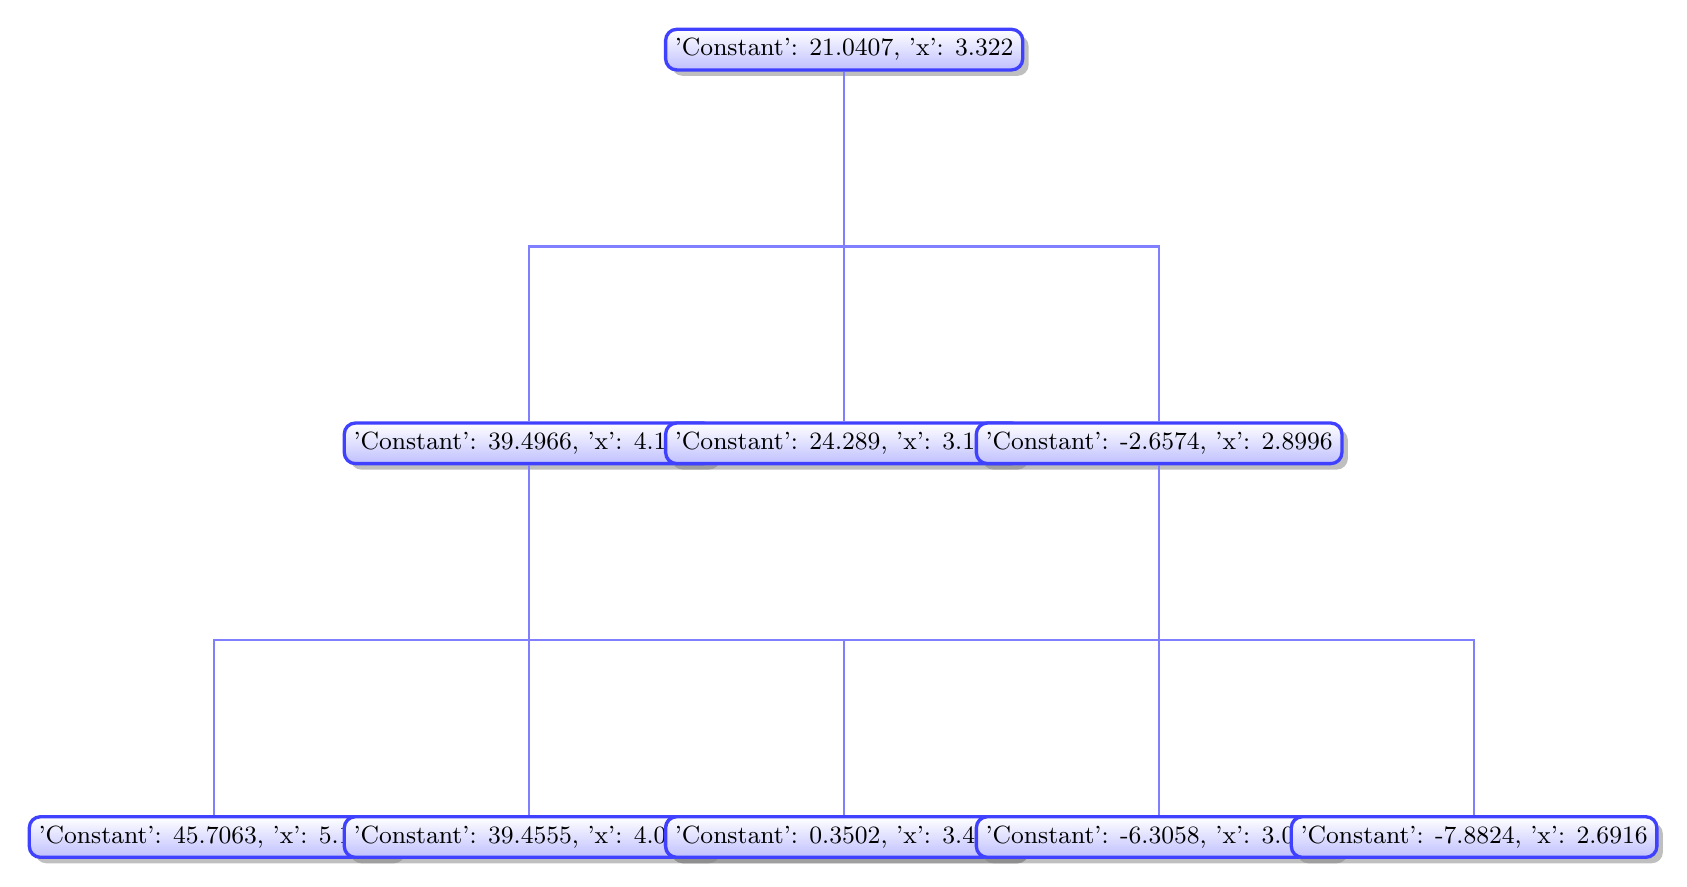
\begin{tikzpicture}
 [font=\small, edge from parent fork down, 
 every node/.style={top color=white, bottom color=blue!25, 
 	rectangle,rounded corners, minimum size=5mm, draw=blue!75,
	very thick, drop shadow, align=center},
 edge from parent/.style={draw=blue!50,thick},
 level 1/.style={sibling distance=4cm},
 level 2/.style={sibling distance=4cm}, 
 level 3/.style={sibling distance=4cm}, 
 level 4/.style={sibling distance=4cm}, 
 level 5/.style={sibling distance=4cm}, 
 level 6/.style={sibling distance=4cm}, 
 level distance=2cm,
 level distance=5cm,
 ]
\node {{'Constant': 21.0407, 'x': 3.322}} %root
child { node {{'Constant': 39.4966, 'x': 4.1694}}  
child { node {{'Constant': 45.7063, 'x': 5.1836}}  
 }
child { node {{'Constant': 39.4555, 'x': 4.0267}}  
 }
child { node {{'Constant': 26.269, 'x': 3.7712}}  
 }
 }
child { node {{'Constant': 24.289, 'x': 3.1251}}  
 }
child { node {{'Constant': -2.6574, 'x': 2.8996}}  
child { node {{'Constant': 0.3502, 'x': 3.4957}}  
 }
child { node {{'Constant': -6.3058, 'x': 3.0951}}  
 }
child { node {{'Constant': -7.8824, 'x': 2.6916}}  
 }
 }
;\end{tikzpicture} 
 \caption{coefficient plot }  \end{figure}
\end{document} 
